\section{Requisitos e arquitetura da solução}
\label{sec:requisitos-arquitetura}

Esta seção reúne o que foi levantado em campo e o desenho que dele decorre. A
ordem é deliberada: primeiro como o processo acontece hoje, depois onde o esforço
se concentra, e só então o que o sistema precisa fazer e como ele se organiza
para fazê-lo. Requisito sem o processo que o origina é afirmação sem lastro, e a
avaliação ao fim do trabalho vai ser feita contra esse processo, não contra o
desenho.

\subsection{Procedimento de levantamento}
\label{subsec:procedimento-levantamento}

O levantamento combinou três fontes de evidência, com pesos diferentes.

A primeira foi uma entrevista estruturada com a servidora responsável pela fase
preparatória no setor de licitações do município estudado, seguida de uma sessão
de validação na qual a especificação já redigida foi lida bloco a bloco para que
ela a corrigisse. A segunda foi a análise de documentos de processos encerrados
cedidos pelo setor: documentos de formalização de demanda, estudos técnicos
preliminares, termos de referência e relatórios de cotação. A terceira foi a
medição desses documentos, descrita adiante.

A distinção entre as três importa e é mantida ao longo do texto. O que a
servidora declarou aparece como declaração; o que os documentos mostram aparece
como medida; e o que foi inferido de um pelo outro aparece como inferência,
sempre identificada. A sessão de validação existiu precisamente para separar
essas camadas, e derrubou três afirmações que até então figuravam como
diagnóstico.

A mais consequente das três merece registro, porque ilustra o risco do método.
A comparação entre as datas de assinatura sugeria que o estudo técnico
preliminar era assinado depois da cotação e ainda assim se referia a ela como
evento futuro, o que foi lido como prova documental de inversão da ordem legal.
A leitura estava errada: existe uma minuta assinada antes, e é dela que vem o
tempo verbal futuro. O desvio real é outro e menor, e está descrito na
subseção~\ref{subsec:processo-hoje}. Anomalia de documento só vira evidência
depois de verificado quantas versões daquele documento existem.

\pendente{Detalhar, quando a avaliação for desenhada por completo, o tamanho e o
critério de seleção do conjunto de documentos analisados, e explicitar que ele é
de conveniência.}

\subsection{O processo de contratação hoje}
\label{subsec:processo-hoje}

O processo começa quando uma secretaria identifica uma necessidade e a formaliza
em um documento de formalização de demanda, informando objeto, quantidade,
período de atendimento e justificativa. Como o município opera por registro de
preços, uma demanda por item de uso comum leva o setor a consultar as demais
secretarias; as listas são somadas e o resultado vira um processo único, para
evitar a multiplicação de procedimentos pequenos. Em um dos processos
analisados, cinco secretarias apresentaram demandas individuais e o processo
consolidado chegou a cento e cinquenta itens.

Formalizada a demanda, a lei prevê a elaboração do estudo técnico preliminar,
que analisa a necessidade, avalia a solução, dimensiona quantidades e estima o
valor \cite{brasil2021lei14133}. Dele deriva o termo de referência, que
estabelece as regras da contratação e é anexado ao edital. Entre os dois entra a
pesquisa de preços.

Duas coisas se afastam do desenho normativo na prática observada.

A primeira diz respeito a quem executa. O estudo técnico preliminar é atribuição
do setor de planejamento, mas quem o redige é o setor de licitações, cabendo ao
planejamento apenas assinar. Corrigir isso não é objetivo deste trabalho: a
correção exigiria habilitar cada secretaria demandante a produzir documento
utilizável por conta própria, o que depende de adesão, treinamento e decisão
administrativa fora do alcance de quem desenvolve o sistema, e não tocaria no
esforço medido, que está inteiramente no setor de licitações. O desvio é
descrito aqui porque explica a carga de trabalho desse setor.

A segunda diz respeito ao número de pesquisas. A legislação prevê uma pesquisa
prévia, destinada a instruir o estudo técnico, e uma cotação definitiva
posterior, que fundamenta o valor estimado. Na prática realiza-se uma cotação
só, cujo resultado alimenta os dois documentos, e o motivo declarado é custo: em
um processo com mais de mil itens, pesquisar preço duas vezes manualmente é
inviável.

Para conciliar isso com a exigência formal, o estudo técnico preliminar tem
ciclo de vida em duas fases. Primeiro é redigida e assinada uma minuta com todas
as seções preenchidas, exceto a estimativa de valor, que aparece redigida no
futuro, declarando que o valor será aferido pela pesquisa a ser realizada. Em
seguida acontece a cotação. Por fim a minuta é retomada e a seção de estimativa
é reescrita no passado, com o valor apurado e as fontes consultadas.

A comparação entre a minuta e a versão final de um mesmo processo confirma o
mecanismo: das doze seções numeradas, onze são idênticas, e apenas a estimativa
de valor difere. É dado de projeto, e não só de diagnóstico, porque descreve
exatamente a transformação que o sistema precisa reproduzir.

\subsection{Onde o esforço se concentra}
\label{subsec:onde-doi}

O município já utiliza um banco de preços comercial, o Banco de Preços, que
agrega bases públicas e privadas. Esse serviço resolve a coleta dos preços,
calcula a média, gera memória de cálculo, monta o mapa comparativo, registra a
procedência de cada preço e emite relatório com mecanismo de verificação de
autenticidade. A coleta, portanto, é problema resolvido, e qualquer proposta que
se apresente como solução para ela chega tarde.

O que esse serviço não faz é interpretar o item. A busca é por palavra: o
operador digita um termo e o sistema devolve todo registro cuja descrição o
contenha, cabendo à pessoa ler candidato por candidato e decidir se o que
apareceu corresponde ao que foi pedido. Os exemplos relatados ilustram o tipo de
erro que isso produz. Uma busca por alface devolveu preços de sanduíche natural,
porque a descrição do sanduíche menciona alface. Uma busca por urna funerária
devolveu também serviços de translado. Uma busca por trator de esteira devolveu
locações cobradas por hora, que são serviço e não equipamento.

Esses relatos foram reproduzidos em ferramenta pública. O catálogo da
ferramenta federal de pesquisa de preços, consultável sem autenticação, foi
submetido a onze consultas em outubro de 2026, e o comportamento observado é o
mesmo descrito pela servidora.

\begin{table}[H]
  \centering
  \caption{Consultas ao catálogo da ferramenta federal de pesquisa de preços}
  \label{tab:consultas-catalogo}
  \begin{ufopaespacosimples}
  \small
  \begin{tabularx}{\textwidth}{@{}llX@{}}
    \toprule
    \textbf{Texto digitado} & \textbf{Sugestões} & \textbf{As primeiras} \\
    \midrule
    alface & 10 & Alfacalcidol; Alfacipermetrina; Verdura in natura \\
    alfase & 0 & --- \\
    hortaliça folhosa & 0 & --- \\
    hortaliça & 10 & Sopa infantil; Mistura para suplementação; Substrato
      agrícola \\
    papel sulfite A4 & 10 & Papel abrasivo; Papel alfa cheque; Papel almaço \\
    sulfite & 10 & Sulfito de sódio; Papel para correspondência \\
    resma papel ofício & 0 & --- \\
    caneta esferográfica azul & 10 & Caneta esferográfica; Caneta indicador \\
    \bottomrule
  \end{tabularx}
  \end{ufopaespacosimples}
  \fonte{Consultas realizadas pelo autor em outubro de 2026, na interface
    pública da ferramenta.}
\end{table}

A leitura é direta: o casamento é de caracteres. Quem procura alface recebe
primeiro um fármaco e um agrotóxico cujos nomes começam com as mesmas letras;
quem erra uma letra, ou usa expressão sinônima para a mesma coisa, não recebe
nada. O comportamento é reproduzível por qualquer leitor, sem credencial, e é o
que converte o relato da servidora em evidência verificável.

É nesse ponto que o sistema atua. Ele recupera candidatos a preço de referência
por proximidade de significado, aplica os filtros que hoje a pessoa aplica de
cabeça, apresenta a evidência que sustenta cada candidato e gera os documentos
da fase preparatória a partir desses mesmos dados.

A medição sobre os processos cedidos sustenta o recorte. Um processo de cento e
vinte itens levou nove dias corridos entre a abertura da pesquisa e o relatório
final; outro, de cento e cinquenta itens, levou vinte e oito. A conformidade
formal, por outro lado, é alta: a exigência de três preços por item foi atendida
com folga mínima, e a totalidade dos preços datados estava dentro da janela de
doze meses. Ou seja, o resultado sai correto, e caro.

\pendente{Acrescentar o número de preços conferidos e a margem mais apertada de
validade quando a seção de avaliação definir como a medição será reportada. Os
valores existem e estão registrados; falta decidir o nível de detalhe que cabe
no artigo.}

\subsection{Regras de negócio}
\label{subsec:regras-de-negocio}

As regras a seguir decorrem da legislação e da prática do setor. Valem
independentemente da existência do sistema, e o sistema não pode contrariá-las.
Apresenta-se aqui o subconjunto que condiciona o desenho; a relação completa
integra a especificação de requisitos que acompanha este trabalho.

\begin{table}[H]
  \centering
  \caption{Regras de negócio que condicionam o desenho da solução}
  \label{tab:regras-de-negocio}
  \begin{ufopaespacosimples}
  \small
  \begin{tabularx}{\textwidth}{@{}lX@{}}
    \toprule
    \textbf{Código} & \textbf{Regra} \\
    \midrule
    RN03 & Demandas de mesmo objeto vindas de secretarias distintas são
      consolidadas em um processo único de registro de preços, preservando-se a
      quantidade de cada uma \\
    RN04 & O termo de referência é derivado do estudo técnico preliminar.
      Divergência entre os dois em campo pareado é motivo de questionamento e
      pode levar ao cancelamento do processo \\
    RN06 & A pesquisa de preços exige no mínimo três preços por item. Com menos
      de três, é obrigatório justificar \\
    RN07 & Um preço só é válido como parâmetro se tiver sido coletado dentro dos
      últimos doze meses \\
    RN08 & Todo preço utilizado deve ter procedência comprovável anexada ao
      processo, na forma do relatório íntegro da pesquisa \\
    RN11 & Preços originados do mesmo evento de contratação não constituem
      observações independentes \\
    RN13 & A unidade de medida do preço de referência deve ser compatível com a
      unidade do item demandado \\
    RN16 & A unidade de medida provém de vocabulário fechado. Embalagem não é
      unidade de medida \\
    RN17 & A busca de preço observa prioridade geográfica: estado, depois
      região, depois âmbito nacional \\
    RN20 & O documento de pesquisa registra o método matemático aplicado, e cada
      preço declara o dispositivo legal que o autoriza como parâmetro \\
    \bottomrule
  \end{tabularx}
  \end{ufopaespacosimples}
  \fonte{Elaborado pelo autor a partir da legislação e do levantamento de campo.}
\end{table}

Duas delas têm evidência direta nos documentos e merecem nota.

A regra RN16 é a que mais restringe a automação. Entre os seis documentos de
demanda analisados, a mesma unidade de medida aparece escrita de quatro formas
diferentes. Não se trata de preciosismo de redação: o sistema de prestação de
contas do tribunal de contas competente aceita um conjunto fechado de unidades e
recusa o que estiver fora dele. Qualquer filtro automático por unidade esbarra
nisso antes de esbarrar em qualquer outra coisa.

A regra RN13, combinada com a anterior, delimita o teto de qualidade da
correspondência entre itens. Em um dos processos analisados, o item demandado
especificava dezoito atributos técnicos, e nenhum dos preços candidatos trazia
descrição que permitisse verificar um único deles. A qualidade da recuperação é
limitada pela qualidade das descrições publicadas, que o sistema não controla, e
isso precisa constar dos resultados como limitação e não como falha de
implementação.

\subsection{Requisitos}
\label{subsec:requisitos}

A especificação completa reúne vinte e duas regras de negócio, trinta e nove
requisitos funcionais e onze não funcionais, com critérios de aceitação, método
de verificação e matriz de rastreabilidade ligando cada requisito à evidência que
o originou. Reproduzi-la aqui ocuparia o artigo inteiro. Esta subseção apresenta
o que o sistema faz, em prosa, e tabula apenas os requisitos classificados como
essenciais.

O sistema tem um único perfil de usuário: o servidor do setor de licitações, que
conduz a fase preparatória e responde pela cotação. Ele domina o processo
administrativo e não tem formação em tecnologia. As demais pessoas envolvidas
aparecem no domínio e não operam o sistema: a secretaria demandante origina a
demanda e a envia como documento, a assessoria jurídica lê as peças exportadas, e
o ordenador de despesa assina.

A decisão por um perfil só foi tomada depois do levantamento e contraria o
desenho inicial, que previa dois. O esforço medido está inteiramente no setor de
licitações, e exigir que as secretarias usem o sistema acrescentaria dependência
de adesão e treinamento fora do alcance deste trabalho sem tocar no que custa
caro. A própria usuária pediu o contrário: que o sistema importasse os documentos
de demanda que ela já recebe.

Em funcionamento, o sistema recebe os documentos de demanda no formato em que já
circulam, extrai deles objeto, itens, quantidades, unidades e secretaria de
origem, e submete o resultado ao operador para correção antes de a demanda entrar
no processo. Quando mais de uma secretaria pede o mesmo item com descrições
divergentes, propõe uma descrição de consenso e devolve a proposta para decisão
do operador; o alinhamento com as secretarias continua acontecendo fora do
sistema, pelos meios já em uso. Em seguida emite a minuta do estudo técnico
preliminar, conduz a pesquisa de preços recuperando candidatos por proximidade de
significado, apresenta-os com a evidência que os sustenta, registra a triagem
feita pelo operador, calcula o valor estimado com memória de cálculo e gera o
mapa de cotação, o estudo técnico em versão final e o termo de referência, todos
em formato editável.

\begin{table}[H]
  \centering
  \caption{Requisitos não funcionais essenciais}
  \label{tab:rnf-essenciais}
  \begin{ufopaespacosimples}
  \small
  \begin{tabularx}{\textwidth}{@{}lXl@{}}
    \toprule
    \textbf{Código} & \textbf{Requisito} & \textbf{Categoria} \\
    \midrule
    RNF01 & Não exigir substituição de sistema em uso pela prefeitura nem
      integração com sistema legado & Projeto \\
    RNF02 & Entregar documentos em formato editável e planilhas em formato de
      uso corrente & Interoperabilidade \\
    RNF03 & A revisão manual de um estudo técnico gerado não deve ultrapassar
      duas horas de trabalho & Usabilidade \\
    RNF04 & Toda afirmação em documento gerado deve ser rastreável até sua
      origem, sem base legal citada sem referência conferível & Confiabilidade \\
    RNF05 & Ser operável por uma única pessoa, sem apoio de equipe de tecnologia
      da informação & Usabilidade \\
    RNF06 & Processar contratação de até mil e quinhentos itens sem degradação
      que inviabilize o uso & Desempenho \\
    RNF08 & Manter trilha de auditoria imutável e consultável, permitindo
      reproduzir o estado de uma pesquisa passada & Confiabilidade \\
    RNF10 & Exigir autenticação individual, com toda ação da trilha de auditoria
      nomeando quem a praticou & Segurança \\
    \bottomrule
  \end{tabularx}
  \end{ufopaespacosimples}
  \fonte{Elaborado pelo autor.}
\end{table}

O requisito RNF10 merece justificativa, já que o sistema tem um perfil só e
alguém poderia concluir que a autenticação sobra. Ela não sobra, por duas razões
independentes. A trilha de auditoria exige registrar quem tomou cada decisão, e
isso só faz sentido se houver quem: trilha anônima vale pouco perante órgão de
controle. E o sistema lida com processo administrativo em curso, cujo valor
estimado ainda não é público.

Duas restrições de projeto completam o quadro. Os documentos precisam sair em
formato editável porque circulam entre setores e são ajustados antes da
assinatura. E a estrutura dos documentos não pode ser inventada: o estudo técnico
obedece a um conjunto de seções vinculadas aos incisos da lei, cada uma
declarando qual dispositivo atende, e a ordem adotada pelo município não coincide
com a ordem dos incisos, de modo que as duas convenções precisam ser respeitadas
ao mesmo tempo.

\subsection{Arquitetura da solução}
\label{subsec:arquitetura}

A arquitetura é apresentada em dois níveis de ampliação, no estilo do modelo
C4\pendente{: conferir a referência primária de Brown antes de citar}. O primeiro
mostra o sistema como caixa única e quem conversa com ele; o segundo abre essa
caixa. Há níveis mais profundos, e eles ficam deliberadamente de fora por
enquanto: descer antes de ter certeza do que cada parte faz produz desenho que
não sobrevive ao primeiro incremento de implementação.

\begin{figure}[H]
  \centering
  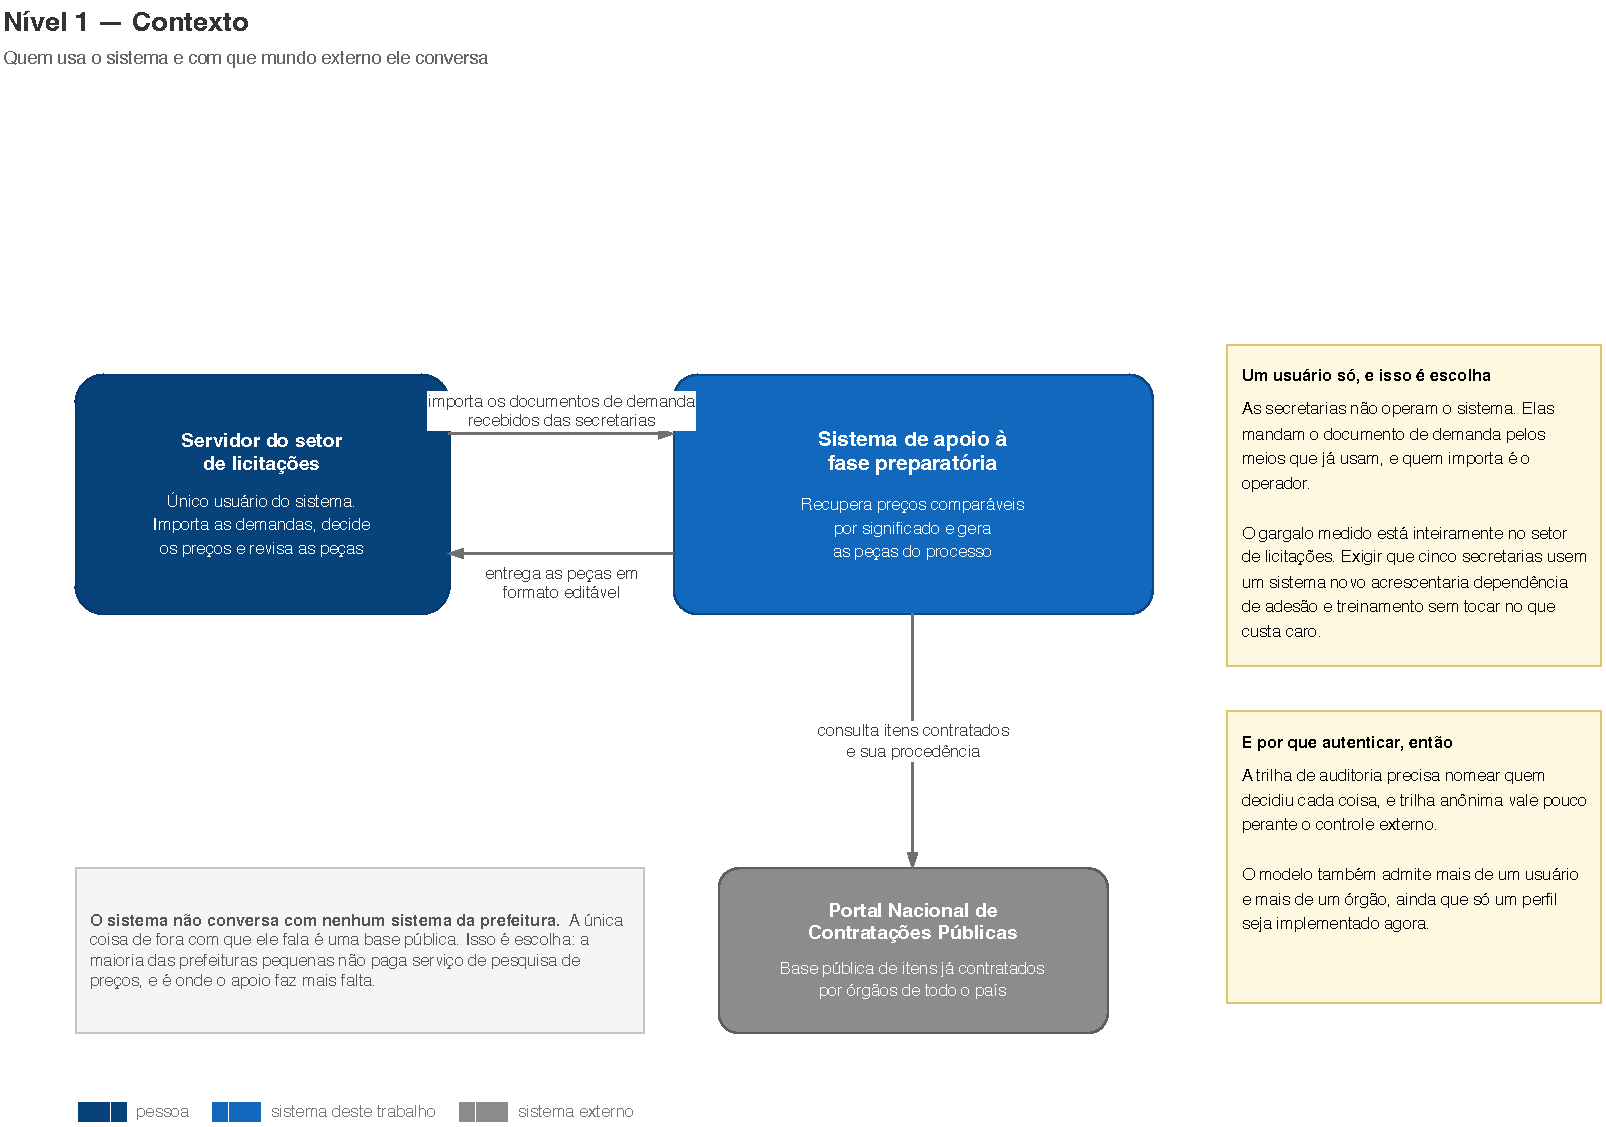
\includegraphics[width=\textwidth]{figuras/arquitetura-nivel1-contexto.pdf}
  \caption{Nível 1 --- contexto: quem usa o sistema e com que mundo externo ele
    conversa}
  \label{fig:nivel1-contexto}
  \fonte{Elaborado pelo autor.}
\end{figure}

No primeiro nível há três participantes. O operador do setor de licitações, o
sistema de apoio, e a base pública de contratações, consultada por interface de
programação. O desenho já decide uma coisa: o sistema não se comunica com nenhum
sistema da prefeitura, e a única fonte externa com que fala é essa base pública.
Isso é escolha, não limitação. O município estudado paga por um serviço comercial
de pesquisa de preços, mas a maior parte das prefeituras de pequeno porte não
tem esse recurso, e é justamente onde o apoio faz mais falta.

\begin{figure}[H]
  \centering
  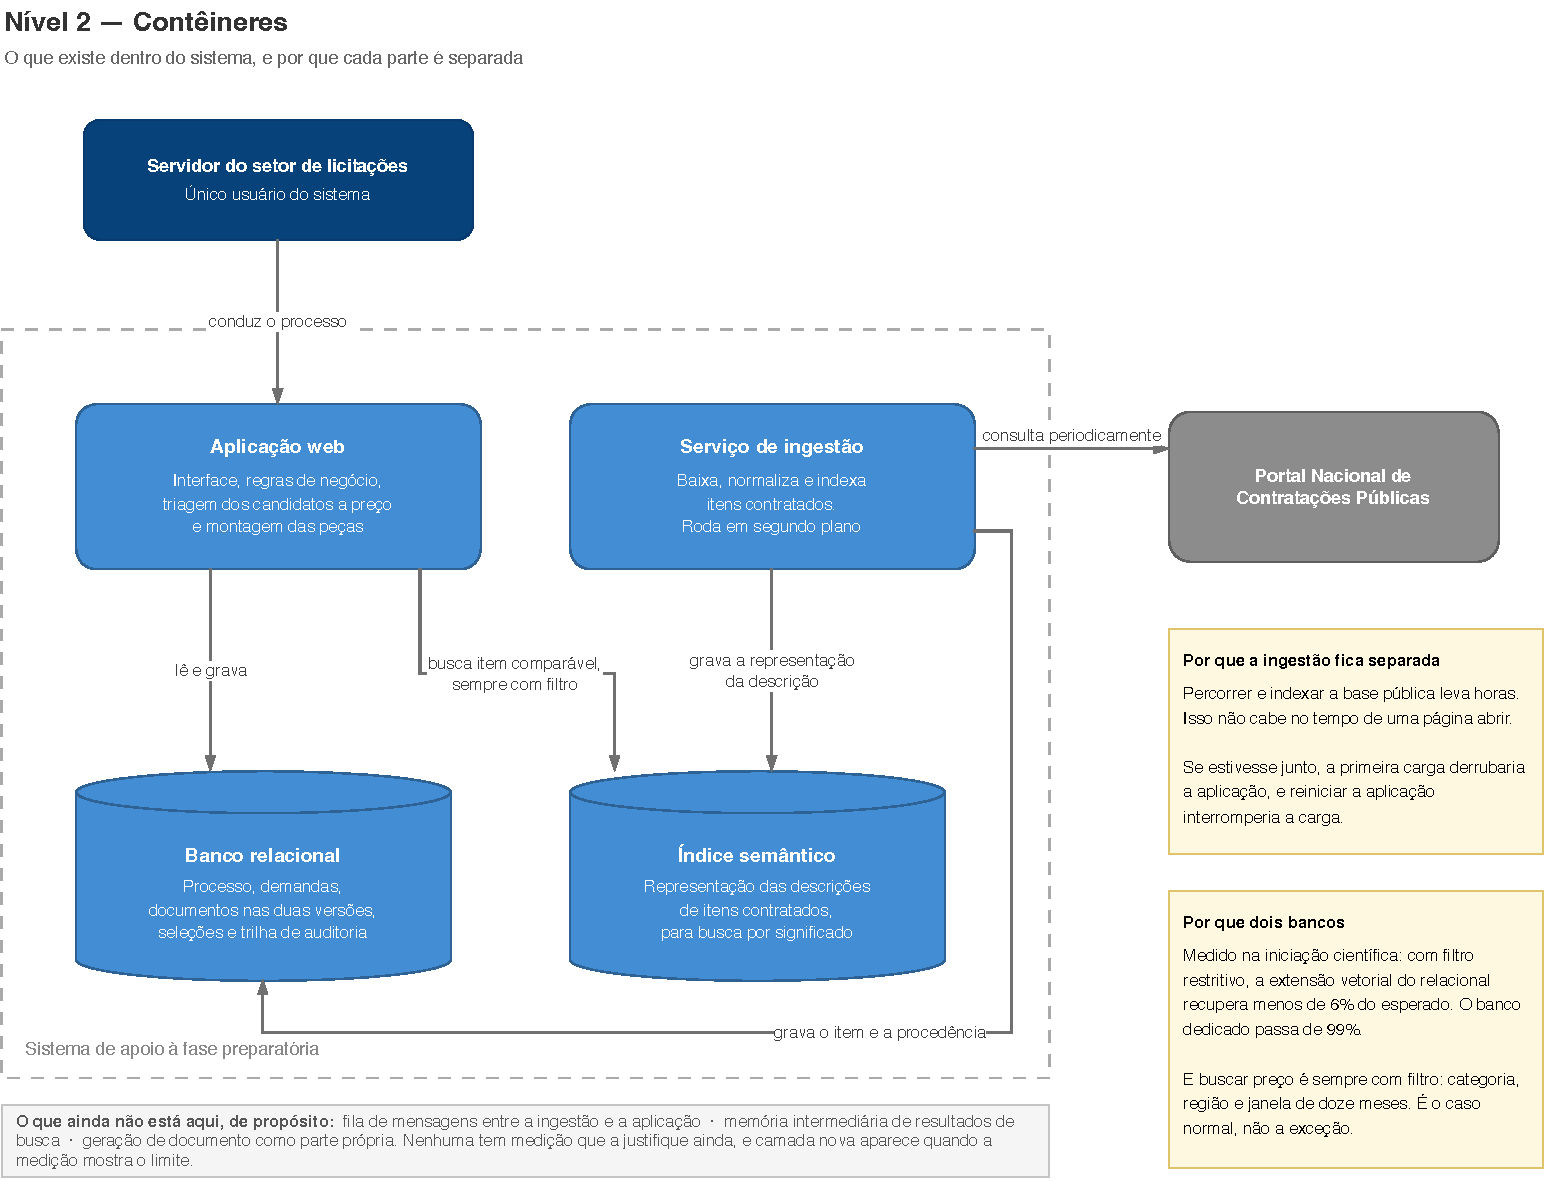
\includegraphics[width=\textwidth]{figuras/arquitetura-nivel2-conteineres.pdf}
  \caption{Nível 2 --- contêineres: o que existe dentro do sistema, e por que
    cada parte é separada}
  \label{fig:nivel2-conteineres}
  \fonte{Elaborado pelo autor.}
\end{figure}

No segundo nível há quatro partes: a aplicação web, um serviço de ingestão, um
banco relacional e um índice semântico. Duas separações estruturam o desenho, e
cada uma tem motivo declarado.

A ingestão fica apartada da aplicação porque percorrer e indexar a base pública é
operação de horas, que não cabe no tempo de resposta de uma requisição. Se
estivessem juntas, a primeira carga degradaria a aplicação, e reiniciar a
aplicação interromperia a carga. O serviço roda em segundo plano, mantém o índice
atualizado e grava, junto de cada preço, a procedência que a regra RN08 exige.

A persistência é dupla porque os dois lados guardam coisas de natureza diferente.
O banco relacional guarda o que precisa de integridade referencial e histórico:
processos, demandas, versões de documento, seleções de preço e a trilha de
auditoria. O índice semântico guarda as representações das descrições, para a
busca por significado. Há medição própria sustentando essa separação, obtida em
iniciação científica anterior a este trabalho: sob filtro restritivo, a extensão
vetorial do banco relacional recuperou menos de seis por cento dos vizinhos
esperados, contra mais de noventa e nove por cento de um banco vetorial dedicado.
A ressalva metodológica é explícita, e consta também da
seção~\ref{sec:metodologia}: trata-se de medição do autor, não de evidência
revisada por pares.

A condição que torna essa medição pertinente é que a busca de preço é sempre
filtrada. Procura-se dentro de uma categoria, numa faixa geográfica e numa janela
de doze meses, por força das regras RN07 e RN17. O cenário medido é o caso
normal de uso deste sistema, e não uma exceção construída.

\begin{figure}[H]
  \centering
  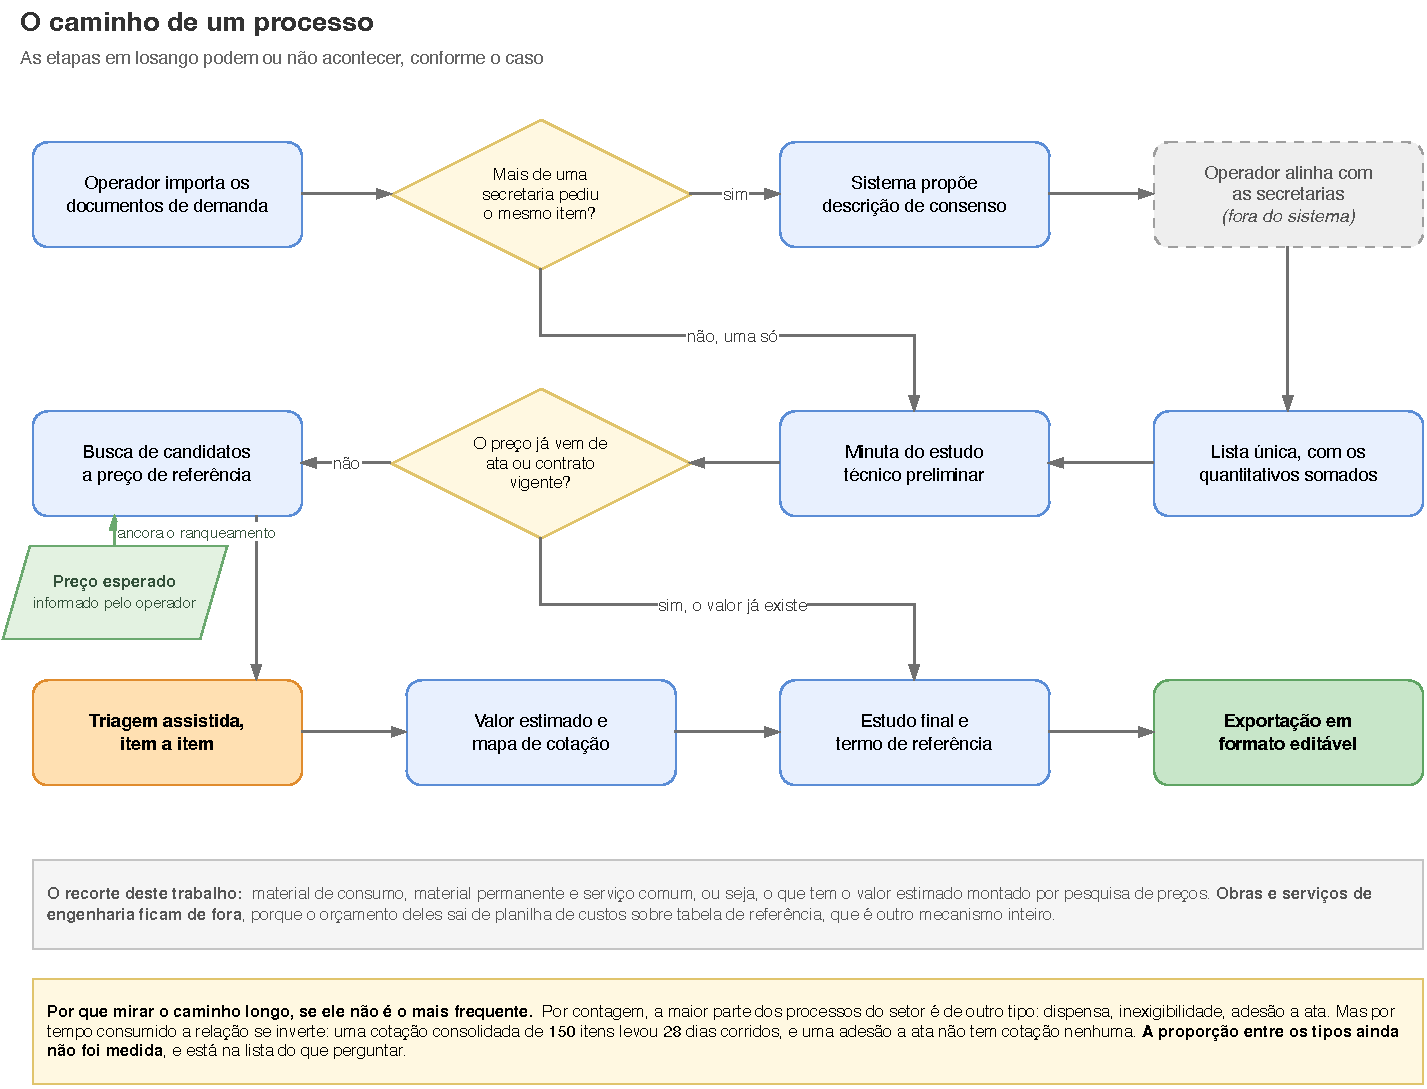
\includegraphics[width=\textwidth]{figuras/arquitetura-fluxo-processo.pdf}
  \caption{O caminho de um processo pelo sistema. As etapas em losango podem ou
    não acontecer, conforme o caso}
  \label{fig:fluxo-processo}
  \fonte{Elaborado pelo autor.}
\end{figure}

O caminho de um processo pelo sistema tem duas etapas condicionais, e isso
precisa ficar explícito porque delimita o alcance do que se promete. A
consolidação só acontece quando mais de uma secretaria pede o mesmo item. E a
pesquisa de preços é pulada quando o preço já vem de ata de registro ou contrato
vigente, caso em que o fluxo segue direto para a emissão das peças.

Uma entrada do fluxo não é etapa do sistema e merece registro: o preço esperado,
informado pelo operador. Observou-se, na demonstração de tela, que a servidora
descarta candidatos antes mesmo de ler a descrição, apenas por implausibilidade
de valor, e que a origem desse número varia entre conhecimento de consumo
cotidiano, cotação pedida a fornecedor local e consulta a mecanismo de busca
comum. A consequência para o desenho é que o ranqueamento tem duas dimensões e
não uma: semelhança do item e proximidade do preço esperado. Elas são exibidas
separadas, e não fundidas em escore único, para que o operador saiba qual das
duas puxou cada candidato para cima.

\subsection{Alcance do que foi modelado}
\label{subsec:alcance}

O setor conduz cerca de dez contratações por semana somando todas as
modalidades, e o caminho modelado não é o mais frequente entre elas. Contratações
de obras e serviços de engenharia ficam fora do escopo, porque seu orçamento é
montado por planilha de custos sobre tabela de referência, que é mecanismo
distinto da pesquisa de preços tratada aqui. Adesões a ata e contratações diretas
também não percorrem o caminho inteiro.

O recorte se justifica pelo tempo, não pela contagem: um processo consolidado de
cento e cinquenta itens consumiu vinte e oito dias corridos, enquanto uma adesão
a ata não tem cotação alguma. A escolha é atacar onde o esforço se concentra.

Registra-se, porém, uma limitação ainda não resolvida: a proporção entre os tipos
de processo não foi medida. Enquanto ela for desconhecida, qualquer ganho que
este trabalho venha a demonstrar vale para o tipo de processo modelado, e não
para a rotina do setor como um todo. A afirmação a ser sustentada nos resultados
precisa carregar essa qualificação.

\subsection{Decisões ainda abertas}
\label{subsec:decisoes-abertas}

As decisões a seguir estão abertas por falta de informação, e não por omissão.
Registrá-las como abertas é preferível a fechá-las cedo e descobrir depois que a
escolha não se sustentava.

\begin{table}[H]
  \centering
  \caption{Decisões de arquitetura em aberto e o que cada uma aguarda}
  \label{tab:decisoes-abertas}
  \begin{ufopaespacosimples}
  \small
  \begin{tabularx}{\textwidth}{@{}lXX@{}}
    \toprule
    \textbf{\#} & \textbf{Decisão} & \textbf{Aguarda} \\
    \midrule
    A1 & Linguagem e arcabouço de desenvolvimento & Não afeta os dois níveis
      desenhados; fechar cedo prende sem necessidade \\
    A2 & Como representar as descrições de item para a busca & Teste com as
      descrições reais, que são curtas e ruidosas \\
    A3 & Política de atualização da ingestão & Medição do volume e do ritmo de
      publicação da base pública \\
    A4 & Onde reside a geração dos documentos & Dimensionar quanto essa parte
      cresce \\
    \bottomrule
  \end{tabularx}
  \end{ufopaespacosimples}
  \fonte{Elaborado pelo autor.}
\end{table}

A decisão A2 é a que mais afeta o resultado do trabalho, e é a próxima a ser
fechada. A A3 depende de uma medição simples sobre a base pública, já planejada.
